% !TeX root = ../main.tex
% Add the above to each chapter to make compiling the PDF easier in some editors.

\chapter{Introduction}\label{chapter:introduction}
\section{Objectives}

Manipulation of objects is one of the most natural action of humankind. Humans never stood and planned about how to manipulate an item. It is an instinct for humans to grab objects in specific ways. Even an infant human can easily manipulate different shapes and colors of objects. Manipulation helps us to use tools, gadgets and provide services. From rehabilitation to service robots, tool usage is vital to enable them to achieve their objective.
Therefore, manipulation skills will be central for robots of any kind. 
Example of our daily manipulation tasks are shown in figure \ref{fig:x manipulation_skills}.

For a complicated manipulation task, first of all, grasping the object is essential. We need first firmly to grab a water bottle to drink it.
Without a firm grasp, the manipulation process may not be successful. 
Nowadays, every kind of robot is helping us produce in the industry. The task robots are responsible for expands from the car manufacturing to high precision microchip producing. On all those tasks, robots are incredibly efficient and precise. However, these tasks' common denominator is that they are repetitive and specialized in a specific process. If a car company decides to manufacture a new car model, the whole process may need to be changed, and the robot's program needs to be hardcoded from zero. Eventually, we want to avoid this redundant task of programming all from zero each time we change the process.

This master's thesis's main objective is to enable robotic 
manipulators to incrementally learn to grasp tools and generalize the learned policy to unseen objects. This procedure promises a robust gripper that can adapt well to unseen objects and environments.. Moreover, rather than hardcoding robot's every move, we take another approach, that the robot learns by itself based on the observation and rewards it receives from the simulation environment. We foresee that through learning-based methods, robots will learn to extrapolate their knowledge to unknown objects and processes \ref{fig:graspseq}.

\begin{figure}[htbp]
    \centering
      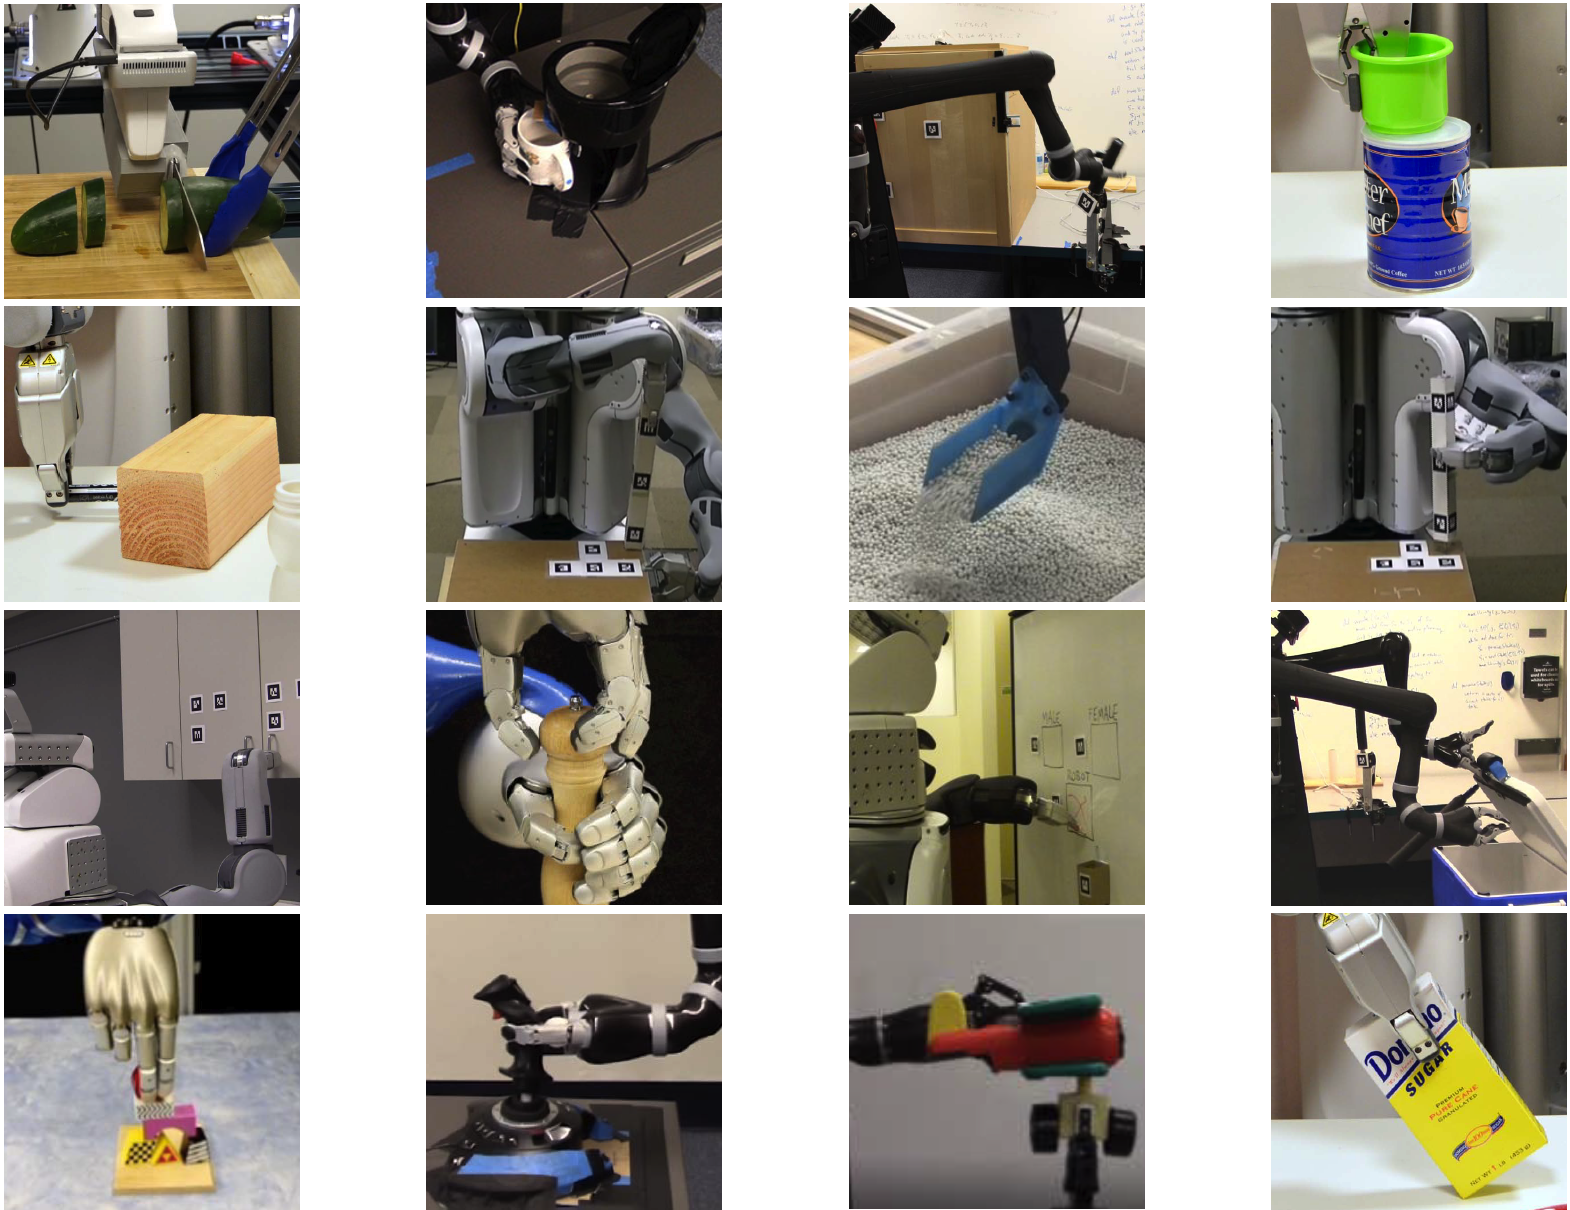
\includegraphics[width=0.8\textwidth]{figures/manipulation_skill}
    \caption{Different manipulation skill adopted to robotic manipulators \cite{Kroemer2019}}
    \label{fig:x manipulation_skills}
\end{figure}

% \begin{figure}[!htbp]
%   \begin{subfigure}{0.49\textwidth}
%       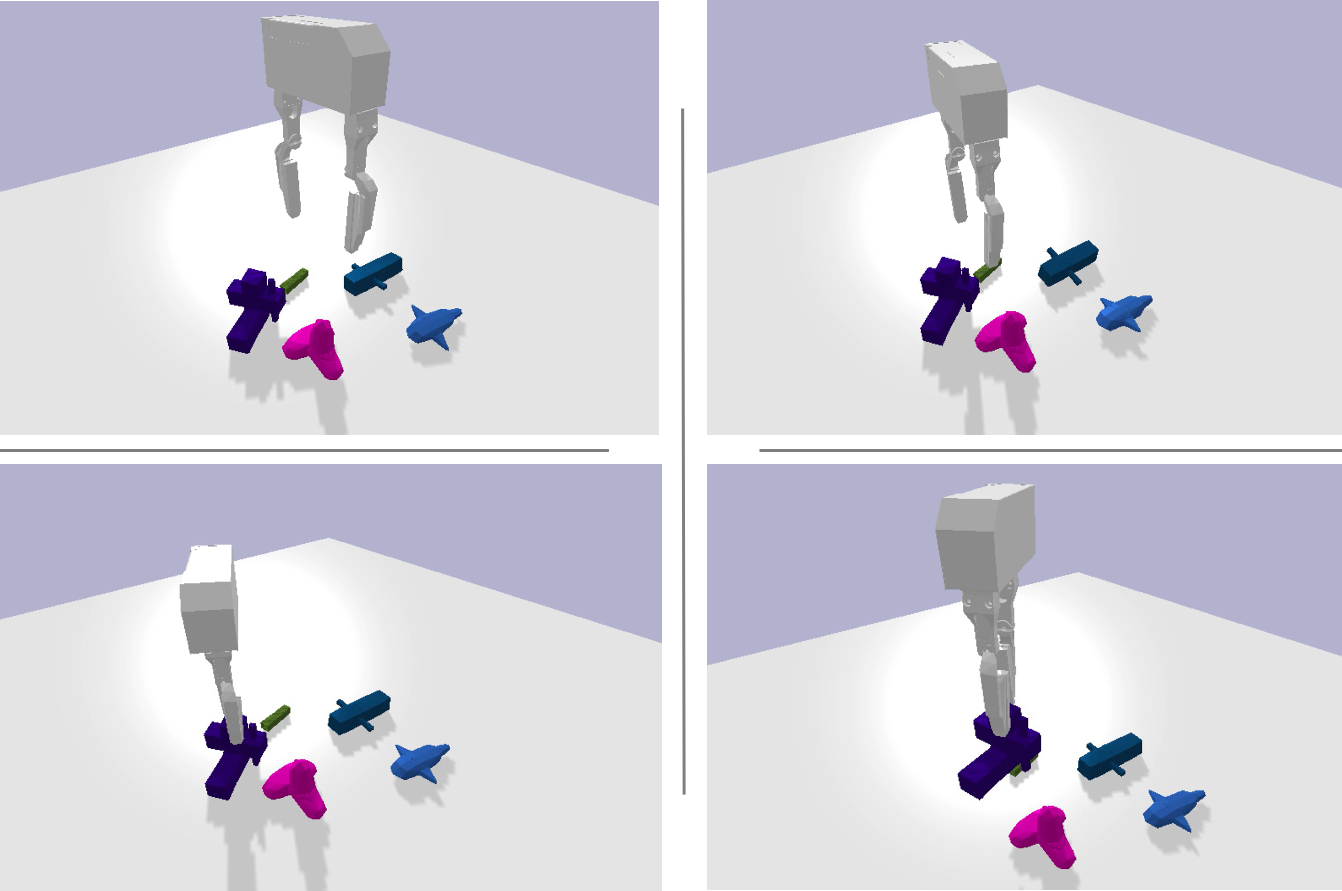
\includegraphics[width=\linewidth]{figures/newfloor}
%       \caption{Grasp sequence in floor scene} \label{fig:table}
%   \end{subfigure}%
%   \hspace*{\fill}   % maximize separation between the subfigures
%   \begin{subfigure}{0.49\textwidth}
%       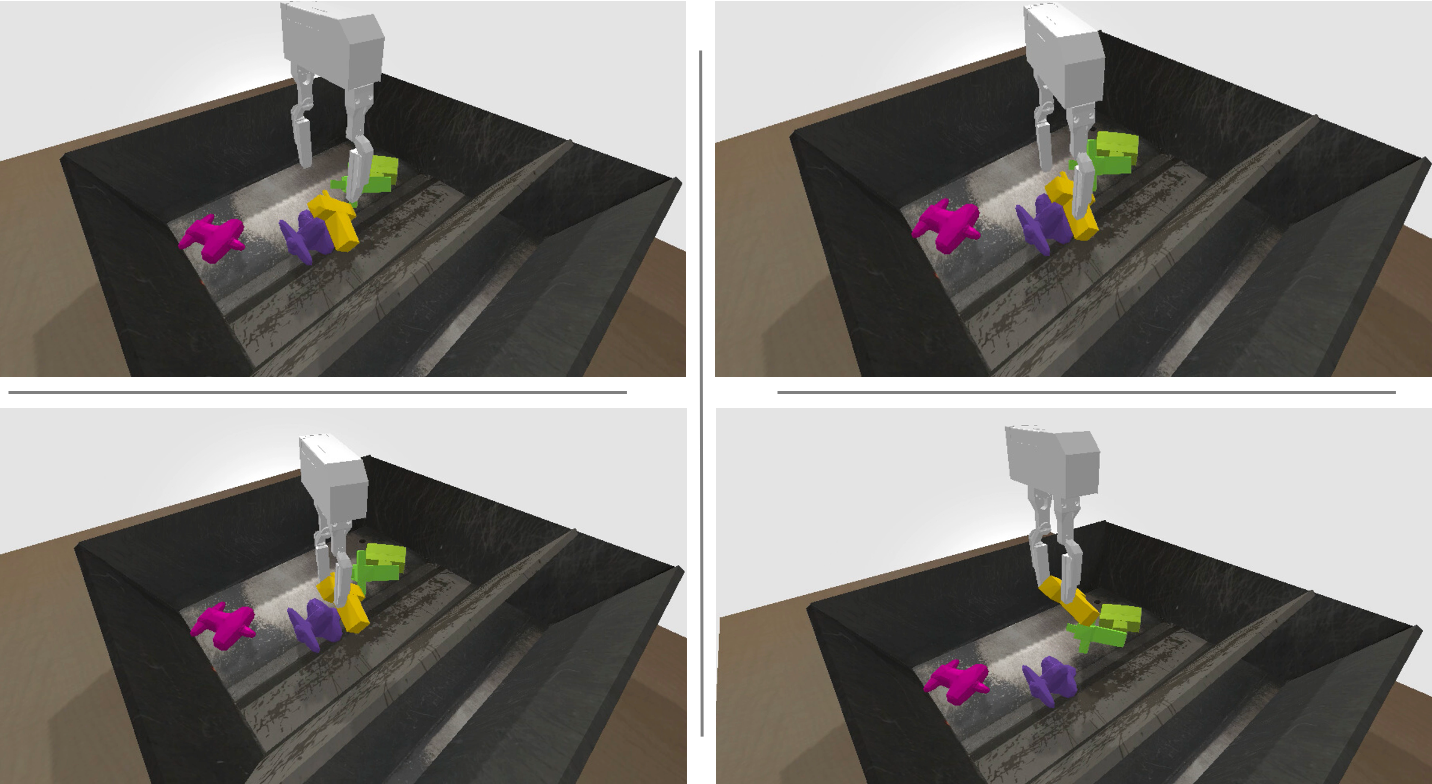
\includegraphics[width=\linewidth]{figures/newtable}
%       \caption{Grasp sequence in table scene} \label{fig:floor}
%   \end{subfigure}%
%   \hspace*{\fill}   % maximize separation between the subfigures    
%   \caption{ Our robot model performs grasping on floor and table scene\label{fig:graspseq}}
% \end{figure}



\begin{figure}[htbp]
  \centering
    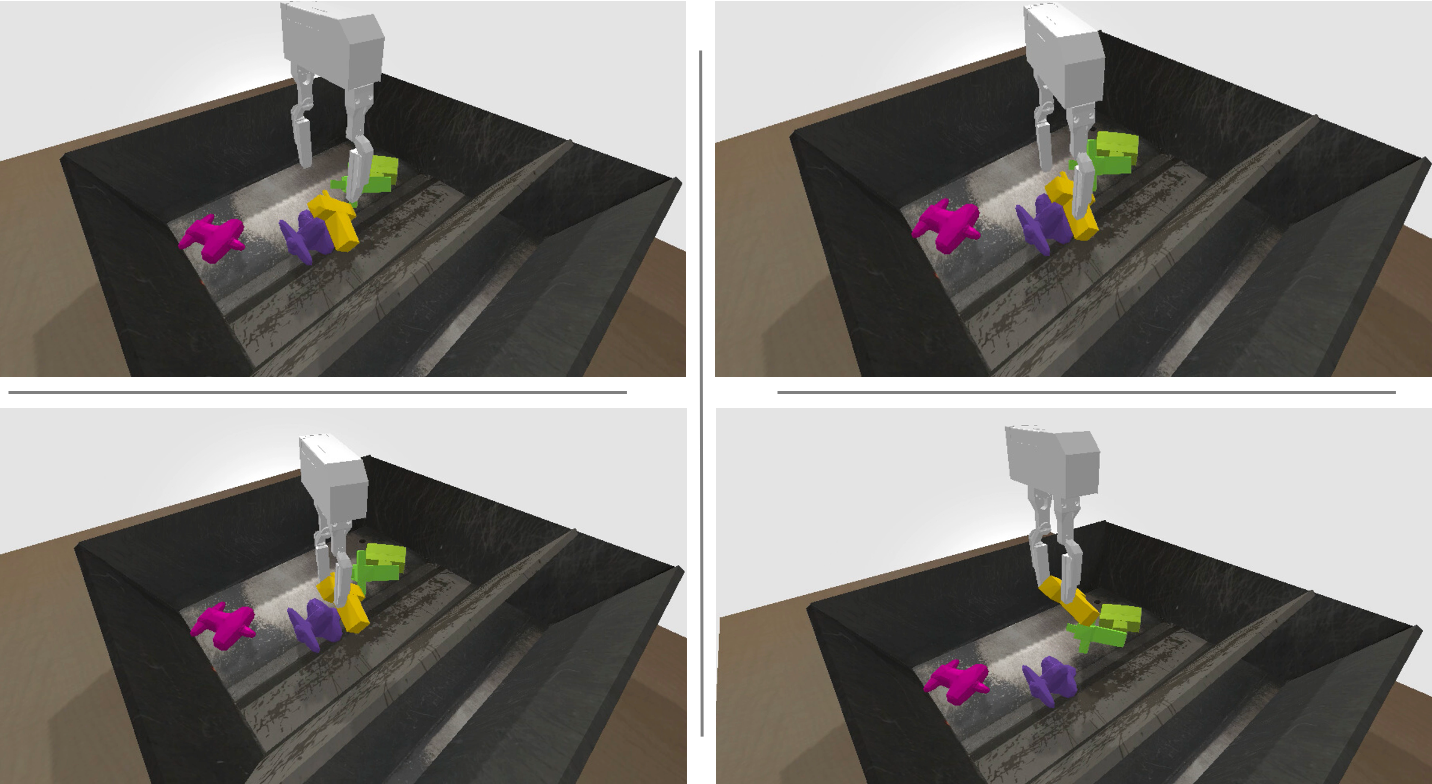
\includegraphics[width=1.\textwidth]{figures/newtable}
  % \caption{Different manipulation skill adopted to robotic manipulators \cite{Kroemer2019}}
  % \label{fig:x manipulation_skills}
  \caption{ Our robot model performs grasping in table scene\label{fig:graspseq}}
\end{figure}

% \begin{figure}[htbp]
%   \centering
%     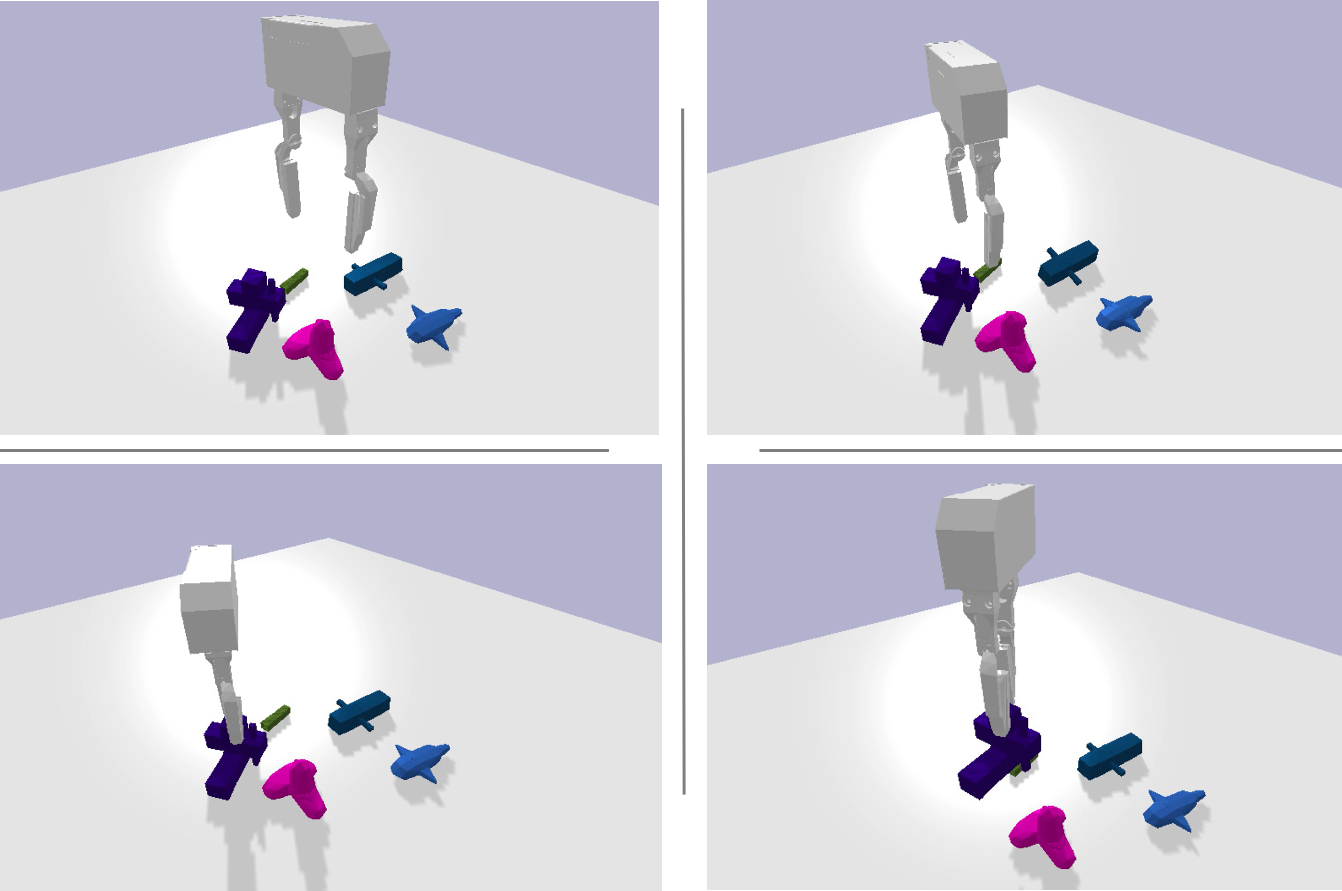
\includegraphics[width=1.\textwidth]{figures/newfloor}
%   \caption{Different manipulation skill adopted to robotic manipulators \cite{Kroemer2019}}
%   \label{fig:x manipulation_skills}
% \end{figure}


% See~\autoref{tab:sample}, \autoref{fig:sample-drawing}, \autoref{fig:sample-plot}, \autoref{fig:sample-listing}, \autoref{fig:tum}, \autoref{fig:tumslide}.
\section{Contribution}

This projects provides two main boiler plate for developers. 
Firstly well documented and tested robot gripper environment based on Open AI Gym interface\cite{openai gym}. 
Gym Environment provides easy to use interface to interact. Moreover, gripper environment complies with the
most standard and well documented libraries such as python3, pybullet and numpy. Secondly, we present a novel implementation of BDQ reinforcement algorithm algorihtm
adopted to most used Stable Baselines project\cite{stable-baselines}.


\section{Challenges}
    \begin{enumerate}
        \item \textbf{Reproducibility} -   Reproducibility is a known issue on machine learning-based approaches. It is never guaranteed to find the global optimum. It is even never guaranteed to find the same local optimum over different trials. Our grasping simulator is random by nature. In our stochastic environment, reproducibility issues can be overwhelming. We cannot verify the hyperparameters’ relative value if the performance changes tremendously over different random seeds. The situation is similar in the low-level,stable-baselines documentation\footnote{\url{https://bit.ly/3jwxhQH}} 
        mention that they cannot even assure the same performance in CPU if the model is trained in GPU. Therefore, we needed to spend more time getting the mean value by running the same model for multiple instances.
        \item \textbf{Hyperparameter Optimization} - Similar to the reproducibility issue, hyperparameter optimization is a very well-known issue in machine learning. No theoretical proofs are saying how hyperparameters need to be tuned. The only solution is to assign the parameters based on some heuristics intuitively. In our work, we used a hyperparameter optimization library to handle this problem. Some trials took up to 80 trials over a week to deliver the most optimized parameters.
        \item \textbf{GPU memory optimization} - GPU memory is the most valuable asset for deep learning applications. If one utilizes the GPU efficiently, one can run more experiments in parallel. Thus, we separated most of our time to fix the encoder or algorithm memory leaks. These leaks clog the GPU memory and lead to unexpected training run shutdowns. That is why we put a lot of effort to minimize the GPU memory usage and maximize memory utilization.
        \item \textbf{Keras and Tensorflow mismatch} - Keras is a high-level, user-friendly interface built on Tensorflow backend. Using both Keras and Tensorflow leads to complicated scenarios, where computation graphs variables can be mixed up. We encountered that the original BDQ algorithm attempted to save the Keras variables used for the auto-encoder implementation with the actual TensorFlow computation graph variables. The overall situation caused a malfunction in the trained model’s save and load functionality. We solved the issue by adequately namespacing every graph variable and tediously saving them in the BDQ algorithm’s save method.
        % \item \textbf{Correct graphics card driver version}
    \end{enumerate}
  
    
% \section{Challenges}
    % \begin{itemize}
    %     \item Reproducibility
    %     \item Hyperparameter tuning
    %     \item Model save and load problems with Tensorlfow
    %     \item Encoder and Model GPU usage
    %     \item 
    % \end{itemize}



% \section{Report Layout}

% \begin{table}[htpb]
%   \caption[Example table]{An example for a simple table.}\label{tab:sample}
%   \centering
%   \begin{tabular}{l l l l}
%     \toprule
%       A & B & C & D \\
%     \midrule
%       1 & 2 & 1 & 2 \\
%       2 & 3 & 2 & 3 \\
%     \bottomrule
%   \end{tabular}
% \end{table}

% \begin{figure}[htpb]
%   \centering
%   % This should probably go into a file in figures/
%   \begin{tikzpicture}[node distance=3cm]
%     \node (R0) {$R_1$};
%     \node (R1) [right of=R0] {$R_2$};
%     \node (R2) [below of=R1] {$R_4$};
%     \node (R3) [below of=R0] {$R_3$};
%     \node (R4) [right of=R1] {$R_5$};

%     \path[every node]
%       (R0) edge (R1)
%       (R0) edge (R3)
%       (R3) edge (R2)
%       (R2) edge (R1)
%       (R1) edge (R4);
%   \end{tikzpicture}
%   \caption[Example drawing]{An example for a simple drawing.}\label{fig:sample-drawing}
% \end{figure}

% \begin{figure}[htpb]
%   \centering

%   \pgfplotstableset{col sep=&, row sep=\\}
%   % This should probably go into a file in data/
%   \pgfplotstableread{
%     a & b    \\
%     1 & 1000 \\
%     2 & 1500 \\
%     3 & 1600 \\
%   }\exampleA
%   \pgfplotstableread{
%     a & b    \\
%     1 & 1200 \\
%     2 & 800 \\
%     3 & 1400 \\
%   }\exampleB
%   % This should probably go into a file in figures/
%   \begin{tikzpicture}
%     \begin{axis}[
%         ymin=0,
%         legend style={legend pos=south east},
%         grid,
%         thick,
%         ylabel=Y,
%         xlabel=X
%       ]
%       \addplot table[x=a, y=b]{\exampleA};
%       \addlegendentry{Example A};
%       \addplot table[x=a, y=b]{\exampleB};
%       \addlegendentry{Example B};
%     \end{axis}
%   \end{tikzpicture}
%   \caption[Example plot]{An example for a simple plot.}\label{fig:sample-plot}
% \end{figure}

% \begin{figure}[htpb]
%   \centering
%   \begin{tabular}{c}
%   \begin{lstlisting}[language=SQL]
%     SELECT * FROM tbl WHERE tbl.str = "str"
%   \end{lstlisting}
%   \end{tabular}
%   \caption[Example listing]{An example for a source code listing.}\label{fig:sample-listing}
% \end{figure}

% \begin{figure}[htpb]
%   \centering
%   \includegraphics[width=0.8\textwidth]{tum}
%   \caption[Something else can be written here for listing this, otherwise the caption will be written!]{Includegraphics searches for the filename without extension first in logos, then in figures.} \label{fig:tum}
% \end{figure}

% \begin{figure}[htpb]
%   \centering
%   \includegraphics[width=0.8\textwidth]{figures/tum}
%   \caption{For pictures with the same name, the direct folder needs to be chosen.} \label{fig:tumslide}
% \end{figure}

% \begin{figure}[!tbp]
%   \centering
%   \subfloat[TUM Logo][The logo.]{\includegraphics[height=0.2\textheight]{tum}\label{fig:tum1}}
%   \hfill
%   \subfloat[TUM Slide][The famous slide.]{\includegraphics[height=0.2\textheight]{figures/tum}\label{fig:tum2}}
%   \caption{Two TUM pictures side by side.}
%   \label{fig:sidebyside}
% \end{figure}

% This is how the glossary will be used.

% \Glspl{ddye}, \gls{r0}, \gls{R0}, and \gls{kdeac}. Also, the \glspl{tum} has many \glspl{computer}, not only one \Gls{computer}. Subsequent acronym usage will only print the short version of \glspl{tuma} (take care of plural, if needed!), like here with \gls{tuma}, too. It can also be --> \glsdisp{tum}{hidden}\footnote{Example for a hidden TUM glossary entry.} <--.
